\section{Bearing Selection}

This section details the process in selecting bearings from the SKF catalogue. However, it is up to you to do your own research and attend the lectures to understand and determine the most appropriate bearings for your design problem.

\subsection{Bearing Types and Locating Bearings}

\begin{framed}
  \vspace{1cm}
    \begin{center}
      {\fontsize{50}{60}\selectfont ?}\\
      Own Research \& Lectures
    \end{center}
  \vspace{1cm}
\end{framed}

%\marginnote{Deep-Groove Ball \\ 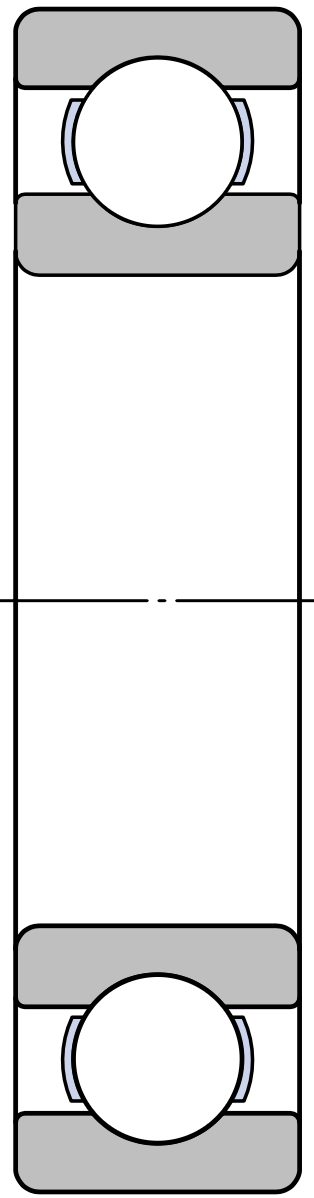
\includegraphics[width=0.06\textwidth]{single-deep-groove-ball-bearing.png}}

%\vspace{3cm}

%\marginnote{Angular Contact Bearing \\ 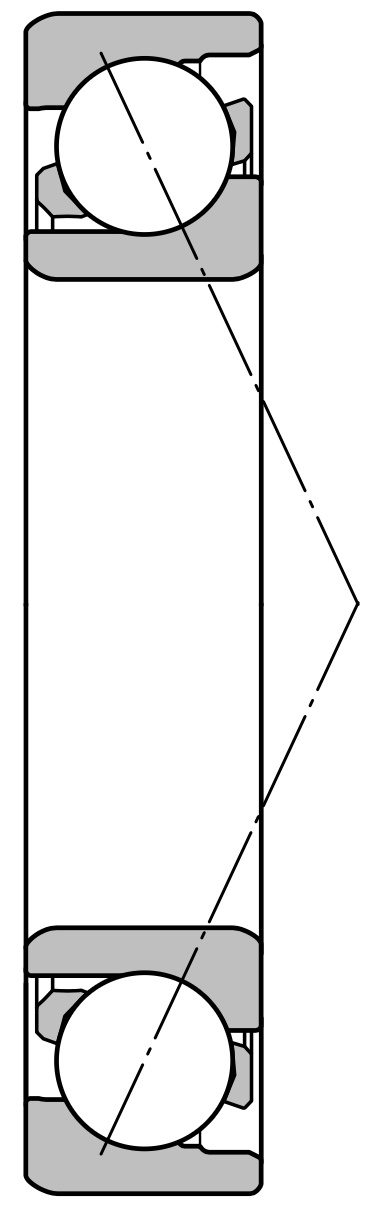
\includegraphics[width=0.07\textwidth]{angular-contact-bearing.png}}

%\vspace{3cm}

%\marginnote{Taper Roller \\ 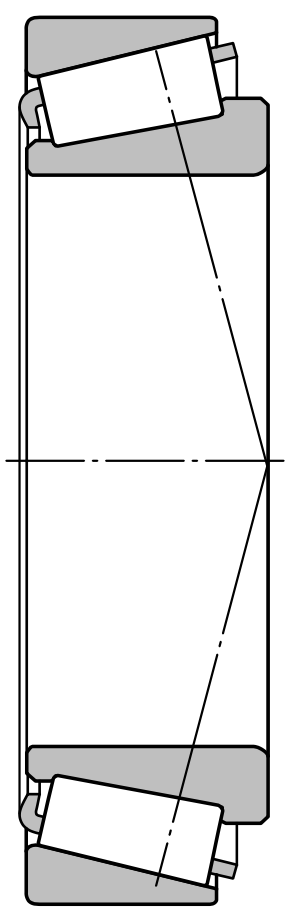
\includegraphics[width=0.07\textwidth]{taper-bearing.png}}

%\vspace{3cm}

%\marginnote{Cylindrical Roller \\ 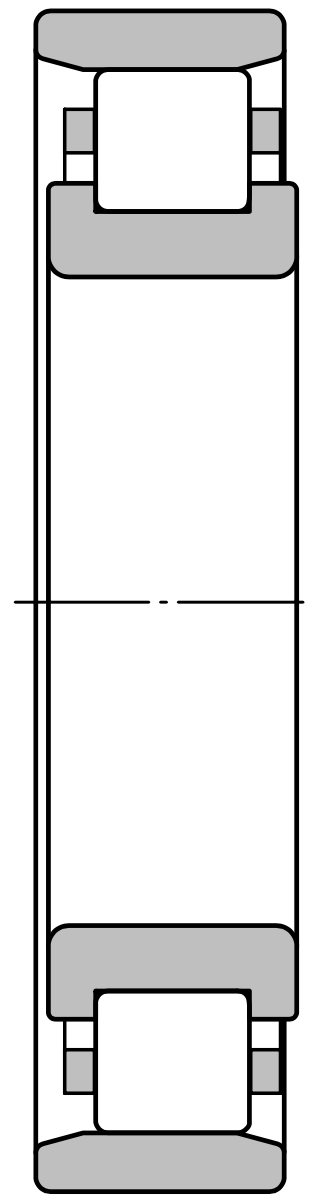
\includegraphics[width=0.07\textwidth]{cylindrical-roller-bearing.png}}

%\vspace{3cm}

%\marginnote{Y-Bearing \\ 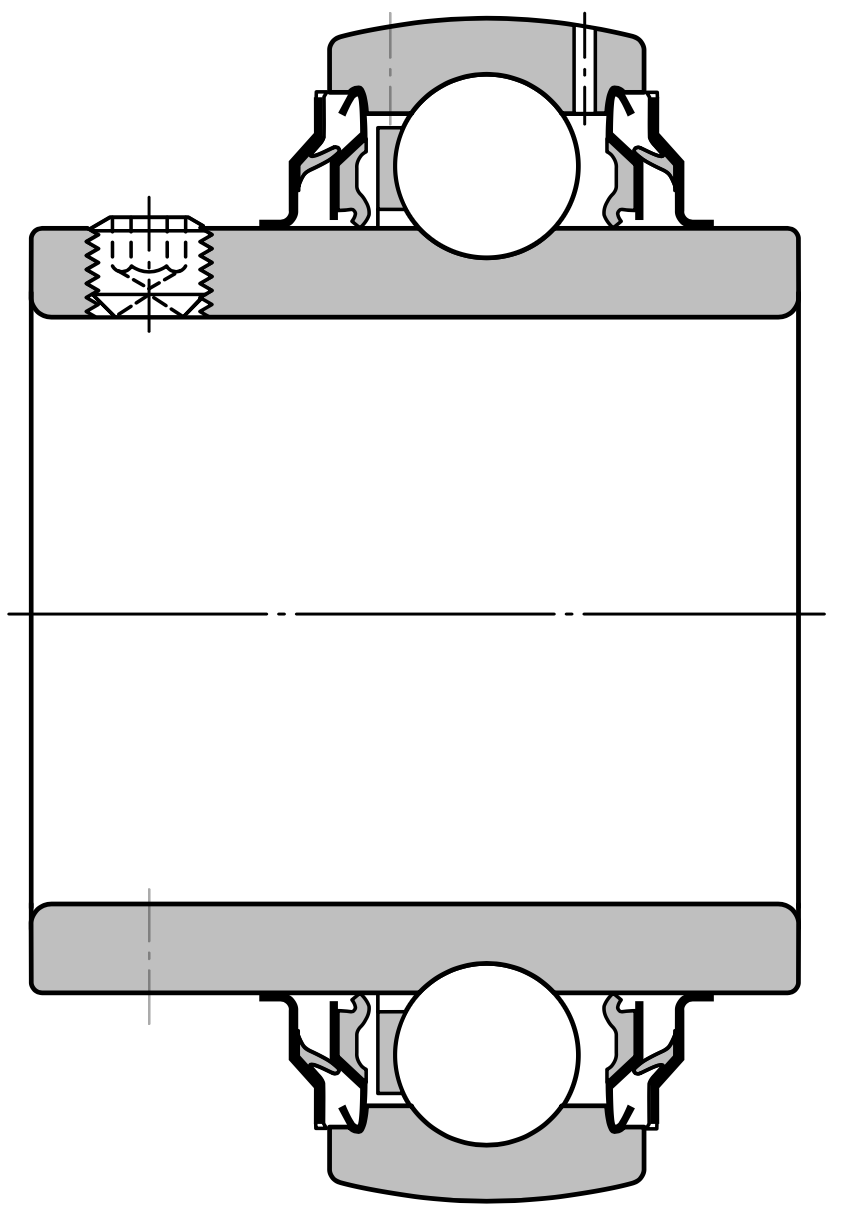
\includegraphics[width=0.2\textwidth]{y-bearing.png}}

%\vspace{3cm}

%\subsection{Locating Bearings}

%\begin{framed}
%  \vspace{2cm}
%    \begin{center}
%      {\fontsize{50}{60}\selectfont \faQuestion{}}\\
%      Research Required
%    \end{center}
%  \vspace{2cm}
%\end{framed}

%\marginnote{\it float}

%\marginnote{\it stepped shaft}

%\marginnote{\it fillet radius}

%\marginnote{\it spacer}

%\marginnote{\it undercut}

%\marginnote{\it pre-load}

\subsection{Bearing Calculations} 

Once you have decided upon the bearing arrangement for your shaft, we can use SKF's bearing selection process to determine the size of bearing that is required. Manufacturers often provide a selection process for their bearings, which they have developed over years of experience in designing and manufacturing their products. The SKF process requires us to determines the basic dynamic \(C\) and static \(C_0\) load ratings that we require for our bearings, which are in accordance of ISO 281:2007 and ISO 76:2006, respectively.


Lets\marginnote{Basic Static Load Rating (\(C_0\))}  start with calculating the basic static load rating for a bearing. This can be calculated using Equation~(\ref{equ-basic-load-rating}) and is where the equivalent static load \(P_0\) is multiplied by a safety factor \(S_0\).

\begin{equation}
  C_0 = P_0 S_0
  \label{equ-basic-load-rating}
\end{equation}

Thus, we need to know both \(P_0\) and \(S_0\).

The\marginnote{Equivalent Static Load (\(P_0\))} calculation for \(P_0\) is dependent upon the type of bearing you're looking to selecting. In the case of a deep-groove ball bearing, \(P_0\) is calculated by:

\begin{equation}
  \text{Calculate } P_0 = 0.6F_r+0.5F_a \text{ then if, } P_0 \le F_r \text{ we set, }P_0 = F_r
\end{equation}

This\marginnote{Safety Factor (\(S_0\))} is then multiplied by the Safety Factor (\(S_0\)), which is selected based on the shafts operating condition.

\begin{itemize}
  \item 0.5 for smooth and shock free
  \item 1.0 for normal
  \item 1.5 for shock and vibration
\end{itemize}

Now\marginnote{Basic Dynamic Load Rating (\(C\))}  we have calculated \(C_0\), we can move onto the basic dynamic load raring (\(C\)), which is calculated through the re-arrangement of the following equation:

\begin{equation}
  L_{10} = \left(\frac{C}{P}\right)^p
  \label{equ-bearing-life}
\end{equation}

\noindent{} Where:

\begin{description}
  \item[\(L_{10}\)] Is the number of revolutions at constant speed that 90\% of bearings tested will complete or exceed before the first evidence of failure develops. This is usually standardised to 1,000,000 cycles in accordance with ISO 281:2007.
  \item[\(C\)] basic dynamic loading rating (\si{\kilo\newton})
  \item[\(P\)] equivalent dynamic bearing load (\si{\kilo\newton})
  \item[\(p\)] bearing factor
  \begin{itemize}
    \item Ball Bearing, \(p=3\)
    \item Roller Bearing, \(p=\frac{10}{3}\)
  \end{itemize}
\end{description}

Thus, to calculate \(C\), we need to know both \(L_{10}\) and \(P\).

To\marginnote{life rating (\(L_{10}\))} determine the life rating (in cycles),

\begin{equation}
  L_{10} = \text{Hours of Operation} \times \text{rpm} \times 60
\end{equation}

With\marginnote{Equivalent Dynamic Bearing Load (\(P\))} \(L_{10}\) now known, we can focus our attention onto \(P\). The calculation for \(P\) is dependent upon the type of bearing you're looking to selecting. In the case of a deep-groove ball bearing (SKF p.316).

\begin{equation}
  P = XF_r + YF_a
\end{equation}

To determine the coefficients \(X\) and \(Y\), we need to find the calculation factors \(f_0\) and \(e\).

From the catalogue, \(f_0\) is calculated using:

\begin{equation}
  f_0 = \frac{F_a}{C_0}
\end{equation}

And \(e\) can be found using the look-up table on page XX in the catalogue. In this case, \(e=0.22\). With these values, we can then decide on, which equivalent dynamic bearing load calculation we require (SKF p.316). One example is:

\begin{equation}
 \text{if, }\frac{F_a}{F_e}\le e \Rightarrow P=F_r \text{ else, } \frac{F_a}{F_e}\ge e \Rightarrow P=XF_r+YF_a
\end{equation}

Once we have \(P\), we can calculate \(C\) be re-arranging the life rating equation (Equation~\ref{equ-bearing-life}). 

\begin{equation}
  \sqrt[p]{L_{10}}\times P = C
\end{equation} 

With\marginnote{Finding a Bearing} \(C_0\) and \(C\) calculated, it is then just a case of looking through the bearing tables and finding a bearing that meets these criteria.

\subsection{Example: Deep Groove Ball Bearing Selection}

A deep groove ball bearing is needed to support a \SI{15}{\kilo\newton} radial and \SI{3}{\kilo\newton} axial loading rotating at \SI{30}{rpm}, on a shaft of \SI{30}{\milli\metre} diameter. The bearing will operate in a smooth-running environment without shock loading, and must be reliable for \SI{5000}{\hour} of operation.

From this description, we can quickly ascertain that:

\begin{itemize}
  \item Deep Groove Ball. Therefore, \(p=3\)
  \item Running speed \(\ge \SI{10}{rpm}\). Therefore, the dynamic load rating is required \(P=XF_r+YF_a\)
  \item Smooth running, vibration free and low shock loading. Therefore, the safety factor \(S_0\) is 1.
  \item \(L_{10} = 5000 \times 60 \times 30 = 9,000,000\) cycles 
\end{itemize}

\marginnote{Equivalent Static Load (\(P_0\))} Using the SKF catalogue, the equivalent static bearing load is given by:

\begin{equation}
  P_0 = 0.6F_r+0.5F_a \text{ then if, } P_0 \le F_r \text{ we set, }P_0 = F_r
\end{equation}

\noindent{} Hence, for this case, \(P_0\) is:

\begin{equation}
  P_0=0.6F_r+0.5F_a = 0.6\times\SI{15}{\kilo\newton} + 0.5\times\SI{3}{\kilo\newton} = \SI{10.5}{\kilo\newton}
\end{equation}

\noindent{} As \(P_0 \le F_r \), we set \(P_0 = F_r = 15\si{\kilo\newton} \).

Now\marginnote{Basic Static Load Rating (\(C_0\))} we can calculate our static load rating \(C_0\) using:

\begin{equation}
  C_0=P_0S_0
\end{equation}

\noindent{} And for our case, \(C_0\) becomes:

\begin{equation}
  C_0= \SI{15}{\kilo\newton} \times 1 = \SI{15}{\kilo\newton}
\end{equation}


Having\marginnote{Equivalent Dynamic Load (\(P\))} calculated \(C_0\), we can move onto calculating the equivalent dynamic load \(P\) so that we can attain the basic dynamic load rating \(C\):

\begin{equation}
  P = XF_r + YF_a
\end{equation}

To determine the coefficients \(X\) and \(Y\), we need to find the calculation factors \(f_0\) and \(e\).

From the catalogue, \(f_0\) is calculated using:

\begin{equation}
  f_0 = \frac{F_a}{C_0} = \frac{3\si{\kilo\newton}}{15\si{\kilo\newton}} = 0.2
\end{equation}

And \(e\) can be found using the look-up table on p.315 in the catalogue. In this case, \(e=0.22\). With these values, we can then decide on, which equivalent dynamic bearing load calculation we require (SKF p.316). 

\begin{equation}
 \text{if, }\frac{F_a}{F_r}\le e \Rightarrow P=F_r \text{ else, } \frac{F_a}{F_r}\ge e \Rightarrow P=XF_r+YF_a
\end{equation}

Therefore, in our case:

\begin{equation}
  \frac{F_a}{F_r}=\frac{3\si{\kilo\newton}}{15\si{\kilo\newton}}=0.2
\end{equation}

\noindent{} and this value is \(\le e\). Thus, 

\begin{equation}
  P=F_r=15\si{\kilo\newton}
\end{equation}

Now\marginnote{Equivalent Dynamic Load Rating (\(C\))} we have all the information we need to determine the equivalent dynamic load rating \(C\) by re-arranging the life rating equation (Equation~\ref{equ-bearing-life}). 

\begin{equation}
  \sqrt[p]{L_{10}}\times P = C = \SI{31.2}{\kilo\newton}
\end{equation}

Now looking through the available bearings in the catalogue and knowing we have to fit onto a \SI{30}{\milli\metre} shaft, two bearings are potentially suitable:

\begin{itemize}
  \item 6306 ETN9
  \item 6406
\end{itemize}

Looking into more detail of the designations of the bearings reveals that ETN9 means that the bearing is reinforced. This is likely to be an over-specification for our application. Therefore, we shall select 6406.

%\subsection{Bearing Selection -- Roller Bearing Example}

%A locating roller bearing is needed to support a 60\si{\kilo\newton} radial and 25\si{\kilo\newton} axial loading rotating at 100\si{rpm}, on a shaft of 75\si{\milli\metre} diameter. The bearing will operate in a normal environment, and must be reliable for 11,000\si{\hour} of operation.

%\begin{itemize}
%  \item Roller. Therefore, \(p=\frac{10}{3}\)
%  \item Running speed \(\ge 10\si{rpm}\). Therefore, the dynamic load rating is required.
%  \item Normal running environment. Therefore, the safety factor \(S_0\) is 1.
%  \item \(L_{10} = 11,000 \times 60 \times 100 = 66,000,000\) cycles 
%\end{itemize}

%\marginnote{Basic Static Load Rating} [TO DO]

%\marginnote{Equivalent Dynamic Load \(P\)} Looking through the SKF catalogue, we identify the equation for \(P\) for locating bearings (p.594).

%\begin{equation}
%\text{If } \frac{F_a}{F_r} \leq e \text{ then } P=F_r \text{ else } P=0.92F_r+YF_a
%\end{equation}

%\begin{equation}
%  \frac{F_a}{F_r}=\frac{25\si{\kilo\newton}}{60\si{\kilo\newton}} = 0.417 > e
%\end{equation}

%To determine \(Y\), we look up the value in the respective SKF table (p.593). In this case, \(Y=0.6\). Thus, \(P\) becomes:

%\begin{equation}
%  P=0.92F_r+0.6F_a=70.2\si{\kilo\newton}
%\end{equation} 

%\marginnote{Basic Dynamic Load Rating \(C\)} Now we have \(P\), we can calculate the basic dynamic load rating \(C\).

%\begin{equation}
%  \sqrt[p]{L_{10}}\times P = C = \sqrt[\frac{10}{3}]{66,0000,000}\times 70,200=246\si{\kilo\newton}
%\end{equation}


%Looking through the SKF tables, we can find a range of suitable bearings with NUP designated bearings able to take axial loads. Focusing on these bearings, two options are available to us:

%\begin{itemize}
%  \item NUP 135 ECP
%  \item NUP 2135 ECP
%\end{itemize}
